\newpage

\ifdefined\DIPLOMA
    \subsection{Теоретические основы управления шаговыми двигателями}
\else
    \section{Теоретические основы}
\fi

\subfile{src/common_definitions}

\newpage
\subsubsection{Физические процессы в шаговом двигателе}
Если не учитывать насыщение магнитной системы, то для статического синхронизирующего
момента $M(\theta)$ справедливо равенство \cite[стр. 82]{Chilikin}:

\begin{equation}
\label{step_motor_torque_common}
    M(\theta)
    = \frac{dW_r}{d\theta_m}
    = p \frac{dW_s}{d\theta}
    = \frac{1}{2} p I_{\textit{ст}} \frac{dL_{\textit{ст}}}{d\theta}
        + \frac{1}{2} p I_{p} \frac{dL_{p}}{d\theta}
        + \frac{1}{2} p I_{\textit{ст}} I_{p} \frac{dL_{\textit{р-ст}}}{d\theta}
\end{equation}

где $I_{\textit{ст}}, I_{p}$ - установившиеся значение токов статора и ротора соответсвенно, А

$L_{\textit{ст}}(\theta)$ - индуктивность статора, Гн

$L_{p}(\theta)$ - индуктивность ротора, Гн

$L_{\textit{р-ст}}(\theta)$ - взаимоиндукция ротора и статора, Гн

Частота собственных упругих колебаний ротора \cite[гл 3.1]{Chilikin} при малых
отклонениях от положения устойчивого положения позволяет получить сторогую оценку
механической подвижности системы и является ее мерой.

\begin{equation}
\label{step_motor_torque_without_load_and_with_unstable_rotor}
    M(\theta)
    = - M_{m} \sin{\theta}
    = - M_{m} \sin({p \theta_{M}})
\end{equation}

\begin{equation}
\label{step_motor_dynamic_move_equation}
    J \ddot{ \theta_{M} } + M_{m} \sin({p \theta_{M} } ) = 0
\end{equation}

При малых отклонениях от положения равновесия таких что:
\begin{equation}
    \sin{\theta} \thickapprox 0
\end{equation}

\begin{equation}
    \label{rotor_like_harmonical_oscilator_equation}
    \ddot{\theta} + \frac{p M_{m}}{J} \theta = 0
\end{equation}

\begin{equation}
    \label{friquent_for_rotor_self_oscilating}
    \omega = \sqrt{ \frac{p M_{m}}{J} }
\end{equation}

Процесс изменения тока в обмотке шагового двигателя при ШИМ-управлении \cite[гл. 6.4, стр. 239]{Chilikin}:

Для случая $0 \le \varepsilon \le \zeta$:
\begin{equation}
    \label{winding_current_with_pwm_control_1}
    i[ n; \varepsilon ] = \frac{ U_1 }{ R }
                            \cdot \{ 1
                                     - \frac { e^{ -\sigma \cdot \varepsilon } } { 1 - e^{-\sigma} }
                                            \cdot [ (1 - e^{-n\sigma})
                                                    - e^{ -(1 - \zeta) \cdot \sigma }
                                                        \cdot ( 1 - e^{-n\sigma + \sigma} )
                                                  ]
                                  \}
                        - \frac{ U_2 }{ R }
                            \cdot \frac {e^{-\sigma}} {1 - e^{-\sigma}}
                            \cdot ( 1 - e^{ -n \cdot \sigma + \sigma } )
                            \cdot ( 1 - e^{ -\sigma + \sigma \cdot \zeta } )
\end{equation}

Для случая $\zeta \le \varepsilon \le 1$:
\begin{equation}
    \label{winding_current_with_pwm_control_0}
    i[n; \varepsilon] =
        \frac{ U_{1} + U_{2} }{ R }
            \cdot \frac{ 1 }{ 1 - e^{-\sigma} }
            \cdot (1 - e^{-\sigma\zeta})
            \cdot (1 - e^{-n\sigma})e^{-\sigma\varepsilon + \sigma\zeta}
        - \frac{ U_{2} }{ R }
            \cdot [ 1 - e^{ -( n - 1 + \varepsilon - \zeta ) \sigma } ]
\end{equation}

где $\varepsilon = \frac{ t }{ T_\textit{шим} }$

$\zeta = \frac{ t_{1} }{ T_\textit{шим} }$

$\sigma = \frac{ T }{ T_\textit{шим} }$

$T = \frac{ L }{ R }$, $\frac{\textit{Гн}}{\textit{Ом}}$

$n$ - число периодов импульсов напряжения,

$t_{1}$ - время подачи напряжения внутри импульса, с

$T_\textit{шим}$ - период ШИМ, с

$t$ - текущее время, с

Максимальное значение тока в импульсе ШИМ согласно (\ref{winding_current_with_pwm_control_1}) при
$\varepsilon = \zeta$ и $U_{2} = 0$:

\begin{equation}
    \label{max_current_in_the_n_pwm_pulse}
    i_{max}[n; \zeta] =
        I_{0}
            \cdot \{ 1
                     - \frac{ e^{-\sigma \cdot \zeta} }{ 1 - e^{-\sigma} }
                       \cdot [ (1 - e^{-n\sigma})
                               - e^{ -(1 - \zeta) \cdot \sigma }
                                    \cdot ( 1 - e^{-n\sigma + \sigma} )
                             ]
                  \}
\end{equation}

где $I_{0} = \frac{ U_{1} }{ R }$, А

Минимальное значение тока в импульсе ШИМ, согласно (\ref{winding_current_with_pwm_control_1}), при
$\varepsilon = 1$ и $U_{2} = 0$:

\begin{equation}
    \label{min_current_in_the_n_pwm_pulse}
    i_{min}[n; \zeta] =
        I_{0}
            \cdot \frac{ 1 }{ 1-e^{-\sigma} }
            \cdot (1 - e^{-\sigma\zeta})
            \cdot (1 - e^{-n\sigma})
            \cdot e^{-\sigma + \sigma\zeta}
\end{equation}

Предел нарастания тока $I_{\textit{шим}.max}$ для данного коэффициента заполнения ШИМ получим из
\ref{max_current_in_the_n_pwm_pulse} в пределе при $n \to \infty$

\begin{equation}
    \label{asymptote_of_current_within_constol_pulse}
    I_{\textit{шим}.max}[\zeta]=
        \lim_{n \to \infty} i_{max} [n; \zeta] =
            I_{0} \cdot \frac{ 1 - e^{-\sigma\zeta} }{ 1 - e^{-\sigma}}
\end{equation}

Скорость нарастания максимумов тока в каждом импульсе оценим как отношение
(\ref{asymptote_of_current_within_constol_pulse}) к (\ref{max_current_in_the_n_pwm_pulse}):

\begin{equation}
    \label{current_grow_estimate}
    \frac{ i_{max}[n; \zeta] }{ I_{\textit{шим}.max}[\zeta] } = 1 - e^{-n \sigma}
\end{equation}

Отсюда мы можем оценить время нарастания тока в течение управляющего импульса:

$$
    n_{ 95 \% } = - \frac{ 1 }{ \sigma }  \cdot \log{(0.05)} \approx \frac{ 3 }{ \sigma }
$$

Передаточная функция шагового двигателя для одного шага при управлении источником
тока \cite[гл. 4.2, ф-ла 4.65]{Kenio}.

\begin{equation}
    \label{step_motor_transfer_function}
    G(s) = \frac{ \omega_{np}^{2} }
                { s^{2} + \frac{D}{J} \cdot s + \omega_{np}^{2} }
\end{equation}

\newpage
\subsubsection{Алгоритмы переключения фаз двигателя}
\label{sec_step_control_algos}

Существует три основных алгоритма переключения фаз шагового двигателя:

\begin{enumerate}
    \item Однофазный
    \item Двухфазный
    \item Полушаговый
\end{enumerate}

\paragraph{Однофазный алгоритм}

\begin{figure}
    \centering
    \begin{minipage}{0.45\textwidth}
        \centering
        \includegraphics[width=\linewidth, keepaspectratio]
                        {./src/pictures/control_algo/one_phase_algo}
        \caption{Диаграмма однофазного режима}
        \label{pic_one_phase_algo}
    \end{minipage}~
    \begin{minipage}{0.45\textwidth}
        \centering
        \includegraphics[width=\linewidth, keepaspectratio]
                        {./src/pictures/control_algo/two_phase_algo}
        \caption{Диаграмма двухфазного режима}
        \label{pic_two_phase_algo}
    \end{minipage}
\end{figure}

Обеспечивается попеременной коммутацей фаз, при этом времена активной работы фаз
не перекрываются, в один момент времени включена только одна фаза. Точки равновесия
ротора для каждого шага совпадают с ``естественными'' точками равновесия ротора у
незапитанного двигателя.

Недостатком этого способа управления является то, что для биполярного двигателя в
один и тот же момент времени используется 50\% обмоток, т.е. в таком
режиме не может быть получен полный момент.

\paragraph{Двухфазный алгоритм}

Временные зоны активной работы перекрываются, две фазы включены в одно и то же
время.

При этом способе управления ротор фиксируется в промежуточных позициях между
полюсами статора и обеспечивается момент, примерно на 40\% больший, чем в случае
одной включенной фазы. Этот способ управления обеспечивает такую же угловую
величину шага, как и первый способ, но положение точек равновесия ротора смещено
на пол--шага. Нужно отметить, что эти положения ротор принимает при работе двигателя,
но положение ротора не может сохраняться неизменным после выключения тока обмоток,
поэтому при включении и выключении питания двигателя ротор будет смещаться на
пол--шага.

Для того, чтобы он не смещался при остановке, необходимо подавать в обмотки ток
удержания. Ток удержания может быть меньше номинального, так как от двигателя с
неподвижным ротором обычно не требуется большого момента.

\paragraph{Полушаговый алгоритм}

\begin{figure}
    \centering
    \includegraphics[width=0.8\linewidth, keepaspectratio]
                    {./src/pictures/control_algo/half_phase_algo}
    \caption{Диаграмма полушагового режима}
    \label{pic_half_phase_algo}
\end{figure}

Этот метод управления достаточно распространен, так как позволяет достич шага с
угловой величиной в два раза меньше номинального. Двигатель с меньшим шагом стоит
дороже и очень заманчиво получить от 100--шагового двигателя 200 шагов на оборот.

Каждый второй шаг запитана лишь одна фаза, а в остальных случаях запитаны две.
Кроме уменьшения размера шага этот способ управления позволяет частично избавиться
от явления резонанса. Полушаговый режим обычно не позволяет получить полный момент.

В основу реализации полушагового режима положен тот факт, что если запитать
одновременно две фазы двигателя, то создаваемый момент будет равен
сумме моментов, обеспечиваемых фазами по отдельности. При этом, если токи в
обмотках одинаковы, то точка максимума момента будет смещена на половину шага.
На половину шага сместится и точка равновесия ротора.

Пиковое значение создаваемого момента при этом будет определяться по формуле
(\ref{half_phase_algo_torque}).

\begin{equation}
    M_\textit{2фаз} = \sqrt{2} M_\textit{1фаз}
    \label{half_phase_algo_torque}
\end{equation}

Преимуществами полушагового алгоритма являются
\begin{itemize}
    \item более высокая разрешающая способность без применения более дорогих
        двигателей
    \item меньшие проблемы с явлением резонанса, резонанс приводит лишь к частичной
        потере момента, что обычно не мешает нормальной работе привода
\end{itemize}

Недостатком полушагового режима является довольно значительное колебание момента от
шага к шагу. В тех положениях ротора, когда запитана одна фаза, момент составляет
примерно 70\% от момента, создаваемого двумя запитанными. Эти колебания могут
явиться причиной повышенных вибраций и шума, хотя они всё равно остаются меньшими,
чем в других режимах.

Способом устранения колебаний момента является поднятие момента в
положениях с одной включенной фазой и обеспечение таким образом одинакового момента
во всех положениях ротора. Это может быть достигнуто путем увеличения тока в
положениях с одной включённой фазой до 141\% от номинального значения
(рис. \ref{pic_torque_diagram}).

\begin{figure}
    \centering
    \includegraphics[width=0.6\linewidth, keepaspectratio]
                    {./src/pictures/control_algo/torque_diag}
    \caption{Величина и направление вектора момента для разных алгоритмов}
    \label{pic_torque_diagram}
\end{figure}

Поскольку ток поднимается только в те моменты, когда включена одна фаза, рассеиваемая
мощность равна мощности в двухфазном режиме при 100\%-ном величине тока от
номинального значения. Однако такое увеличение тока требует более высокого
напряжения питания, что не всегда возможно.

Более предпочтительно для устранения колебаний момента при работе двигателя в
полушаговом режиме снижать ток в те моменты, когда включены две фазы. Для
получения постоянного момента этот ток должен составлять 70,7\% от номинального
значения. Именно такой подход используется в реализации полушагового режима
в управляющей программе.


\newpage
\subsubsection{Управление без ОС}
C помощью (\ref{step_motor_transfer_function}) можно определить пороговую
частоту переключения обмоток, после которой двигатель не сможет запускаться на данной нагрузке.

Собственная частота вращения ротора \cite[гл. 4.2, ф-ла 4.48]{Kenio}

\begin{equation}
    \label{rotor_natural_frequency}
    \omega_{np} = \sqrt{\frac{N_{r}K_{M}I_{p}}{J}}
\end{equation}

Постоянная момента, выраженная из \cite[гл. 4.2, ф-ла 4.52]{Kenio}, при условии
линейности характеристики $r = f(\delta\theta)$

\begin{equation}
    \label{torque_coeff}
    K_{M} = \frac{N_{r}I_{p}\delta\theta}{\tau}
\end{equation}

где $N_{r} = 50$ - число пар полюсов,

$I_{p}$ - ток ротора, А

$\tau$ - статический момент удержания, $H \cdot \textit{м}$

$\delta\theta$ - отклонение от положения равновесия, рад.

Вычислим $K_{M}$ в положении, в котором момент удержания максимален.
В первом приближении он достигается при отклонении от положения равновесия
$\delta\theta = 1.8^{\circ} = 1.8 \cdot \frac{\pi}{180} = 0.031416 ~\textit{рад}$.

Тогда, подставляя паспортные данные $\tau = 0,9 ~\textit{Н} \cdot \textit{м}, I_{p} = 3$ А
в (\ref{torque_coeff}), получим:
\begin{equation}
    \label{first_approximation_moment_coeff}
    K_{M} = 5.26
\end{equation}

Подставляя (\ref{first_approximation_moment_coeff}) в (\ref{rotor_natural_frequency}), получим:
\begin{equation}
    \label{first_approximation_rotor_natural_frequency}
    \omega_{np} = 2,5866 \cdot 10^{2}
\end{equation}

Рассмотрим пусковые возможности двигателя, используя характериистики пускового момента. Из
(\ref{step_motor_transfer_function}) очевидно, что пороговая стартовая частота зависит от момента инерции и
статического момента нагрузки.

C некоторым запасом возьмем пусковые характеристики двигателя для данной нагрузки:
$f_{1}, [\textit{Гц}]$ - максимальная частота следования импульсов при которой двигатель может и
запускаться и останавливаться без сбое и пропуска шагов взятая с некторым запасом.

\paragraph{Линейное ускорение двигателя}
Если функцию зависимости предельной частоты управления от скорости вращения апроксимировать до
линейной с таким запасом, чтобы на графике $f_{max}( \omega )$ она была строго ниже во
всем диапазоне рабочих частот, то мы получим закон изменения частоты управления при линейном
ускорении шагового двигателя без выраженной обратной связи. При этом коэффициент наклона этой
наклонной прямой есть ни что иное как предельное ускорение доступное двигателю.
%% TODO: формулу надо проверить, в ней что то не так
$$
    f_{max}(t) = f_{1} + \beta_{1} \cdot f_{\textit{текущее}}
$$

\paragraph{Линейное торможение двигателя}
Самый простой путь для определения закона управления двигателем при торможении - взять ту же
последовательность, что и при ускорении, но в обратном порядке.
%% TODO: формулу надо проверить, в ней что то не так
$$
    f_{max}(t) = f_{1} + \beta_{2} \cdot f_{\textit{текущее}}
$$
Однако, торможение можно выполнять быстрее, чем ускорение, за счет диссипативных сил,
и коэффициент $\beta_{2}$ несколько больше чем $\beta_{1}$.

\newpage
\subsubsection{Управление с ОС}
\label{sec_feedback_control}
Возможности шагового двигателя могут быть в большой степени расширены при использовании обратной
связи по положению для определения требуемой включённой фазы и времени их включения. В этом случае ШД
будет работать как вентильный двигатель. Кроме исключения ошибок в совершении шага, к положительным
аспектам управления с ОС так же относится более стабилизированное движение ротора, позволяющее достигнуть
более высокой частоты приемистости.

Обратная связь для шагового двигателя в общем виде работает следующим образом:
пусть шаговый двигатель начинает движение. Оптический датчик определяет положение ротора и передает
информацию логическому блоку, который, используя информацию о положении ротора, орпеделяет, какую фазу
нужно включать для текущего положения, и запитывает её. Соотношение между настоящим положением
ротора и фазой (или фазами для микрошаговых режимов), которую следует возбудить, определяется
в терминах угла коммутации.

Смена активной фазы происходит по переходу через целочисленную границу для величины:
$$
    \lfloor ~\theta + \theta_{\textit{ком}}~ \rfloor
$$
Таким образом, с точки зрения управления, при использовании обратной связи шаговый двигатель идентичен
вентильному двигателю постоянного тока.
Частота вращения шагового двигателя с обратной связью определяется величиной нагрузки. Чем больше величина
нагрузка, тем меньше частота вращения.

Угол коммутации предполагает мгновенное нарастание тока в обмотках двигателя, и в этом приближении
угол коммутации при движении в одном направлении может изменяться в пределах $[~1,~2)$.
Однако на практике одношаговый угол коммутации не используется, так как в этом случае нет
уверенности в продолжении движения, поскольку существует момент трения. Предположим ротор движется к
положению равновесия фазы, возбужденной в данный момент. Очевидно, что если статический момент, действующий
на ротор, понижается, то может оказаться так, что момент сухого трения уравняется с моментом,
действующим на ротор. В этом случае ротор не дойдет до угла коммутации следующей фазы и
остановится. В этом случае двигатель остановит вращение. Исходя из этих рассуждений следует
выбирать угол коммутации больше единицы.

Все вышеописанные рассуждения предполагали мгновенное нарастание тока. В реальности же обмотки двигателя
имеют значительную индуктивность, что вызывает отставание по фазе тока от напряжения.
По этой причине необходимо изменить угол коммутации так, чтобы обеспечить переключение активных фаз
в момент, когда угол между нарастанием тока и вектором магнитного поля ротора равен выбранному углу коммутации.

\begin{figure}
    \centering
    \includegraphics[width=0.7\textwidth, keepaspectratio]{./src/pictures/max_step_motor_by_com_angle}
    \caption{Влияние скорости на параметры управления}
    \label{graph_speed_and_angle_comutation}
\end{figure}

Момент шагового двигателя в зависимости от угла отклонения ротора от положения равновесия:
\begin{equation}
    \label{torque_from_rotor_deviation}
    \tau = K_{M} I_{M} N_{r} ( \theta_{i} - \theta_{0} )
\end{equation}

где $K_{M}$ - см. (\ref{torque_coeff}),

$I_{M}$ - ток в обмотке, А

$N_{r} = 50$ - число пар полюсов,

$\theta_{0}$ - положение ровновесия, рад.

$\theta_{i}$ - текущее угловое положение, рад.

С помощью (\ref{torque_from_rotor_deviation}), задав желаемый угол коммутации и
средний (среднеинтегральный) момент, можно получить значение желаемого среднего
(среднеинтегрального) тока, необходимого для поддержания на данном шаге заданного момента.

Параметризуем угол коммутации и обозначим его $\theta_{\textit{ком}}$.
Согласно (\ref{torque_from_rotor_deviation}), момент, действующий на ротор
в начале импульса управления:

\begin{equation}
    \label{moment_to_rotor_at_the_begin_of_control_pulse}
    \tau_{\textit{нач}} = K_{M} I_{M} N_{r} ( \theta_{\textit{ком}} )
\end{equation}

В конце импульса:

\begin{equation}
    \label{moment_to_rotor_at_the_end_of_control_pulse}
    \tau_{\textit{кон}} = K_{M} I_{M} N_{r} ( \theta_{\textit{ком}} - \theta_{\textit{шаг}} )
\end{equation}

Средний момент для этого участка:
$$
    \tau_{\textit{шаг}} = \frac{ \tau_{\textit{нач}} + \tau_{\textit{кон}} }{ 2 }
$$
$$
    \tau_{\textit{шаг}} = K_{M} I_{M} N_{r} ( \theta_{\textit{ком}} - \frac{ \theta_{\textit{шаг}} }{ 2 } )
$$

\subsubsection{Резонансные явления в шаговом двигателе}
Шаговым двигателям свойственен нежелательный эффект, называемый моментным резонансом. Эффект
проявляется в виде внезапного падения момента на некоторых скоростях. Это может привести к пропуску
шагов и выходу из синхронизма. Эффект проявляется в том случае, если частота шагов совпадает с
собственной резонансной частотой ротора двигателя.

При работе двигателя на частоте, совпадающей с резонансной, ротор двигателя колеблется вокруг
положения устойчивого равновесия. При этом возникает провал момента, что приводит к пропуску шагов и
выходу из синхронизма. Без принятия специальных мер, шаговый двигатель при разгоне не может пройти резонансную
частоту. Усиление амплитуды колебаний ротора вокруг положения равновесия вызывает сильные вибрации в
передаточных механизмах, что является причиной избыточного шума и приводит к преждевременному износу
механических деталей привода, нарушениям крепления частей и механизмов. Кроме того,
явление резонанса способно существенно ухудшить точностные характеристики привода, поэтому изучение
резонансных явлений и нестабильностей шагового привода представляет большой практический интерес.

Опыт показывает \cite[гл. 9]{RatmirovIvobotenko}, что существует три вида нестабильности:
\begin{itemize}
    \item \textbf{Низкочастотный резонанс} (частоты $ \le 500 ~\textit{Гц}$).

    \item \textbf{Среднечастотная нестабильность}. Одна из важнейших проблем, которую приходится решать при
            разработке драйвера шагового двигателя и подборе самого двигателя - преодоление данного
            вида резонанса. Он наблюдается в диапазоне шаговых частот 500..1500 Гц и составляет
            1/4, 1/5 максимальной шаговой частоты вращения, см. (рис \ref{pic_step_motor_reisonance_plot})

    \item \textbf{Высокочастотная нестабильность}. Возникает на частотах 1500..2500 Гц, когда двигатель успешно
            проходит область среднечастотной нестабильности.
\end{itemize}

\begin{figure}
    \centering
    \includegraphics[width=0.95\textwidth, keepaspectratio]{./src/pictures/step_motor_reisonance_plot}
    \caption{Резонансные частоты среднечастотной нестабильности}
    \label{pic_step_motor_reisonance_plot}
\end{figure}


% TODO: Я совсем не уверен, что тот резонанс который мы промоделировали является среднечастотной
% нестабильностью, перед дипломом жизненно важно это проверить, либо начисто выпилить отсюда это
% деление на 3
Самое существенное влияние оказывает среднечастотная нестабильность. Она имеет следующие особенности:
\begin{enumerate}
    \item Колебания имеют одну или несколько частотных компонент. Они не связаны простым соотношением с
            шаговой частотой вращения двигателя и имеют более низкую частоту.

    \item При постоянных условиях работы наблюдаются медленно вырастающие колебания.
            Нарушение нормальной работы системы наступает через несколько секунд или даже минут.
            Возможна внезапная потеря синхронизма.

    \item Характеристики нестабильности зависят от схемы и алгоритма управления.
            Существенное влияние оказывает повышение момента инерции системы.
            Большая инерционность увеличивает нестабильность.
\end{enumerate}

%% Без воды ни туды и ни сюды
Для борьбы с резонансом можно использовать различные методы. Одним из них является применение
эластичных материалов при выполнении механических муфт связи с нагрузкой. Эластичный материал
способствует поглощению энергии в резонансной системе, что приводит к затуханию паразитных колебаний.
Существует метод, основанный на свойствах вязкого трения. Выпускаются специальные демпферы, в которых
внутри полого цилиндра, заполненного вязкой кремний-органической смазкой, может вращаться
металлический диск. При вращении этой системы с ненулевым ускорением на диск воздействует момент вязкого
трения, что эффективно демпфирует систему.

Так же существуют электрические методы борьбы с резонансом. Колеблющийся ротор приводит к возникновению в
обмотках статора ЭДС. Закорачивание обмоток, которые на данном шаге не используются, приведет к
демпфированию резонанса.

И, наконец, существуют алгоритмические методы борьбы с резонансом на уровне работы драйвера. Например,
можно использовать тот факт, что при работе с двумя включенными фазами, резонансная частота примерно
на $20\%$ выше, чем с одной включенной фазой. Если резонансная частота точно известна, то ее можно
проходить, меняя режим работы.

Если это возможно, при старте и остановке нужно использовать частоты выше резонансной. Увеличение
момента инерции системы ротор-нагрузка уменьшает резонансную частоту.
Самой эффективной мерой для борьбы с резонансом является применение микрошагового режима.

Возможность потери шаговым двигателем устойчивости на резонансных частотах является его существенным
недостатком и требует детального анализа. Результаты анализа должны быть учтены при выборе
параметроа привода.
